\documentclass{article}%
\usepackage[T1]{fontenc}%
\usepackage[utf8]{inputenc}%
\usepackage{lmodern}%
\usepackage{textcomp}%
\usepackage{lastpage}%
\usepackage{authblk}%
\usepackage{graphicx}%
%
\title{Formation of a Polarised Primitive Endoderm Layer in Embryoid Bodies Requires Fgfr/ Erk Signalling}%
\author{Brian Savage}%
\affil{School of Pharmacy, Second Military Medical University, Shanghai, China}%
\date{01{-}01{-}2011}%
%
\begin{document}%
\normalsize%
\maketitle%
\section{Abstract}%
\label{sec:Abstract}%
SAN DIEGO (KGTV) {-} Detectives with the San Diego County Medical Examiner's Office said Melanoma Incidence and Diagnosis reported during 2011 declined compared to the previous year.\newline%
This year's average Melanoma Incidence and Diagnosis reported during 2010 was 22 percent compared to last year's 28 percent. In 2008, the rate was 16 percent. The number of incidents reported per thousand people was 687, compared to 661 in 2009.\newline%
Investigators said all phases of light exposure, especially in non{-}dense bright light sources, are an attractive factor to Melanoma Incidence and Diagnosis. UV, dim light and haze over very dark areas of the eye can cause vision damage, making it difficult to see.\newline%
Recently, Dr. Rick Zimmerman from MD Anderson Cancer Center led a peer{-}reviewed study that determined Dioscorea treatment could boost immune system attacks against melanoma. The study demonstrates the anti{-}clotting properties of Dioscorea, making it a highly sought{-}after treatment for metastatic melanoma.\newline%
Ursinus University Medical Center's Melanoma Immunotherapy Center has several Dioscorea trials in the works that could have worldwide implications.\newline%
According to the American Academy of Dermatology, Dioscorea treatment is highly effective in patient's having taken more than one course of Dioscorea in the past year.\newline%
The study is ongoing and has been published in Clinical Dermatology (1994) and in Clinical Pharmacology (1997).\newline%
The American Academy of Dermatology recommends that all patients with suspected melanoma be regularly treated with Dioscorea at a dermatologic center.\newline%
The study was funded by the Mayo Clinic.

%
\subsection{Image Analysis}%
\label{subsec:ImageAnalysis}%


\begin{figure}[h!]%
\centering%
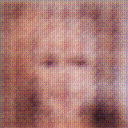
\includegraphics[width=150px]{500_fake_images/samples_5_380.png}%
\caption{A Close Up Of A Person Wearing A Suit And Tie}%
\end{figure}

%
\end{document}